\documentclass[main.tex]{subfiles} 
\begin{document}

\section{Mangfold i naturen}
Ved endt opplæring skal eleven kunne
\begin{itemize}[noitemsep]
\item forklare hovedtrekkene i evolusjonsteorien og gjøre rede for observasjoner som støtter teorien
\item beskrive oppbygningen av dyre- og planteceller og forklare hovedtrekkene i fotosyntese og celleånding
\item gjøre rede for celledeling og for genetisk variasjon og arv
\item forklare hovedtrekk i teorier for hvordan jorda endrer seg og har endret seg gjennom tidene, og grunnlaget for disse teoriene
\item undersøke og registrere biotiske og abiotiske faktorer i et økosystem i nærområdet og forklare sammenhenger mellom faktorene
\item observere og gi eksempler på hvordan menneskelig aktivitet har påvirket et naturområde, undersøke ulike interessegruppers syn på påvirkningen og foreslå tiltak som kan verne naturen for framtidige generasjoner
\item gi varierte eksempler på hvordan samer utnytter ressurser i naturen
\end{itemize}

\subsection{Evolusjonsteorien}
Evolsjonsteorien er en vitenskapelig teori som forklarer og predikerer naturlige fenomener. Frem til 19 århundre, var det antatt at arter forble uforandret siden de ble skapt. Forskningen til Charles Darwin banet veien for dagens forståelse, der arter kan forandres gjennom \emph{naturlig og kunstig seleksjon}, og ved å \emph{tilpasse} seg til sine omgivelser.
\newline\newline
Mennesker har over mange generasjoner utvalgt og oppdrett ønskede egenskaper, gjennom prosessen som kalles \textbf{kunstig seleksjon}. Darwin argumenterte at en tilsvarende prosess forekommer i naturen. \textbf{Naturlig seleksjon} er en prosess der individer som har visse arvelige egenskaper overlever og reproduserer ved et høyere andel enn andre individer på grunn av disse egenskapene. Over tid kan naturlig seleksjon øke organismens tilpasningsevne til deres omgivelser. Hvis omgivelsene og miljøet forandrer, eller individer flytter til en ny omgivelse, naturlig seleksjon kan resultere i tilpasning til disse nye omgivelsene, som noen ganger gir \textbf{opphav} til nye arter.
\newline\newline
Alle levende organismer er utsatt for konkurranse for ressurser, men også predasjon\footnote{Predasjon, defineres bredt som at en organisme spiser hele eller deler av en annen organisme.}. Naturlig seleksjon forekommer ofte ved interaksjon av organismer med andre organismer, så vel som interkasjon av orgranismer med deres fysiske omgivelser.
\newline\newline
Blant direkte observasjoner av evolusjonære forandringer er insekten Serinethinae (eng.: Soapberry bug). I et studie \cite{cabo92}, ble fremvist at insektens ``nebb'' ble lengere når den måtte forandre sine spisevaner. En pågående eksempel på naturlig seleksjon som har en stor dramatisk påvirkning på mennesker er evolusjon av antibiotika resistente bakterier. En annen type bevis for evolusjon kommer fra analysering av likheter mellom forskjellige organismer. En tredje type bevis for evolusjon er fossiler \footnote{Bevarte rester eller spor av organismer fra fjern fortid.}. Bevarte fossiler dokumenterer et mønster av evolusjon, som viser at tidligere organismer var forskjellige fra dagens organismer and at mange arter har utdødd.
\newline\newline
En forståelse for evolusjon gir oss en nærmere tilknytning til resten av skapninger på jorden, hvor vi alle er lenket sammen gjennom jordens utvikling og utforming.
\begin{sidewaysfigure}
    \centering
    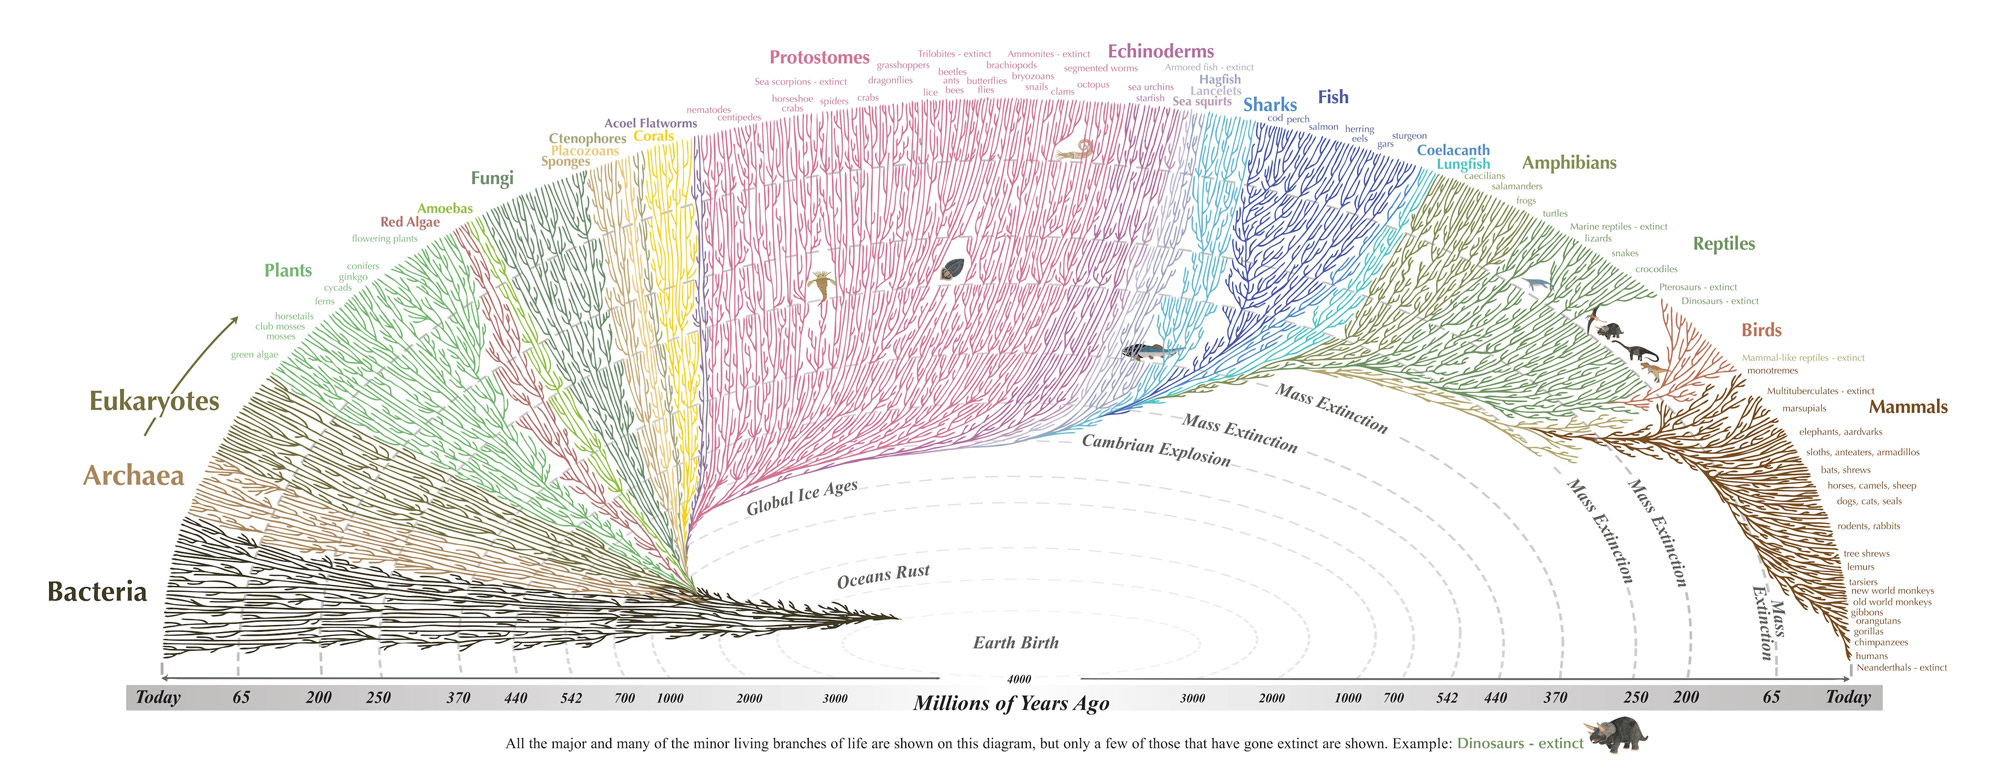
\includegraphics[scale = 0.37]{../figures/utviklingavliv.jpg}
    \caption{Utvikling av liv og forbindelsene mellom arter. Kilde: evogeneao.com}
\end{sidewaysfigure}

\subsection{Celler og oppbygging av celler}
Alle organismer består av celler. Akkurat slik atomer er grunnleggende i kjemi, er celler på tilsvarende vis i biologi. De enkleste levende organismer er enkelt cellede organismer, mens vi mennesker og andre komplekse organismer er flercellede organismer.
\newline\newline
\textbf{Cellemembranen} huser cellens indre membraner, som er detaljert arrangert og deler cellen i flere kamre, også kalt \emph{organeller}.
\newline\newline
\textbf{Cellekjernen} har blant annet \textbf{kromosomer}, som besitter gener i form av \textbf{DNA}.
\newline\newline
\textbf{Cellevegg} finnes hos noen type celler utenfor cellemembranen og gir beskyttelse til cellen, og også som en filtrerings mekanisme. Finnes ofte hos planter og alger, men ikke dyr.
\newline\newline
\textbf{Celledeling}
\begin{figure}[h!]
\centering
    \begin{subfigure}{.5\textwidth}
    \centering
    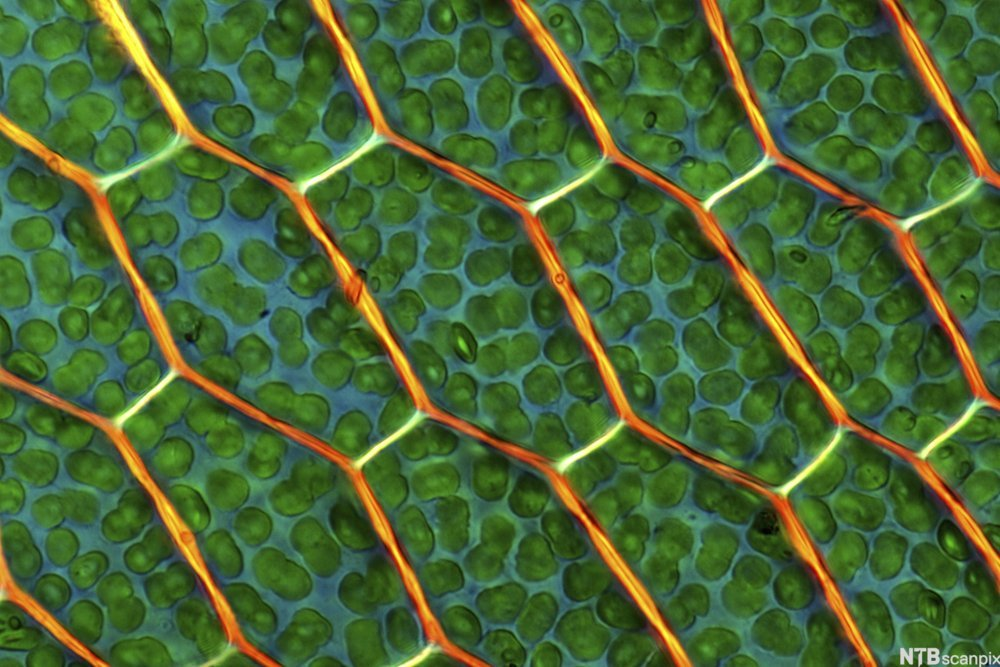
\includegraphics[scale = 0.5]{../figures/cellevegg.jpg}
    \caption{Moseceller med tydelige cellevegger. Kilde: Ndla}
    \end{subfigure}%%
    \begin{subfigure}{.5\textwidth}
    \centering
    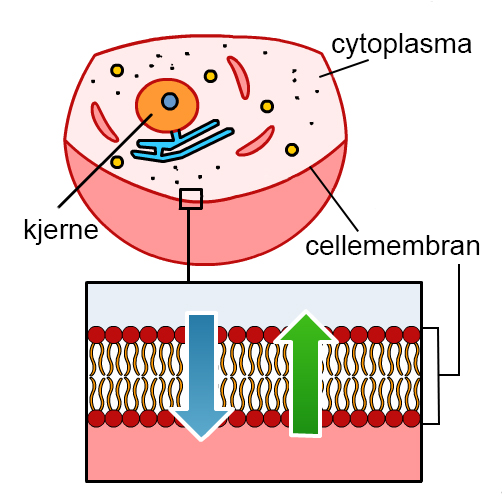
\includegraphics[scale = 0.25]{../figures/cellemembran.jpg}
    \caption{En dyrecelle. Kilde: Ndla}
    \end{subfigure}
    %\begin{subfigure}{.5\textwidth}
    %\centering
    %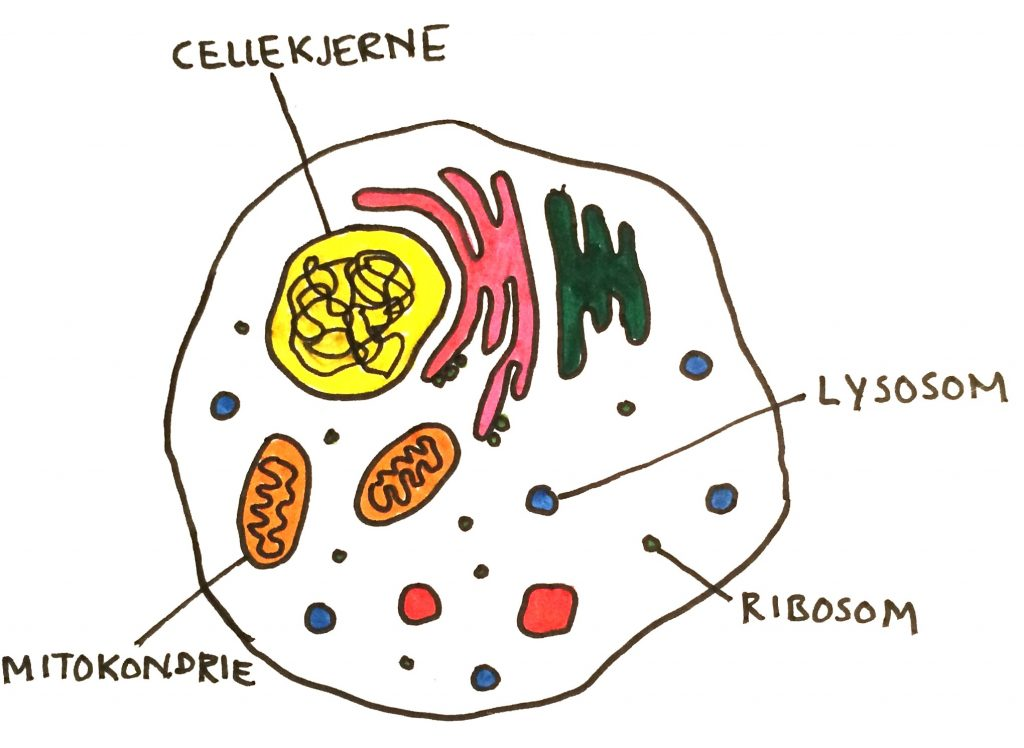
\includegraphics[scale = 0.3]{../figures/cellekjernen.jpg}
    %\caption{Oversikt over cellekjernen. Kilde: omhelse.no}
    %\end{subfigure}%%
    \begin{subfigure}{.5\textwidth}
    \centering
    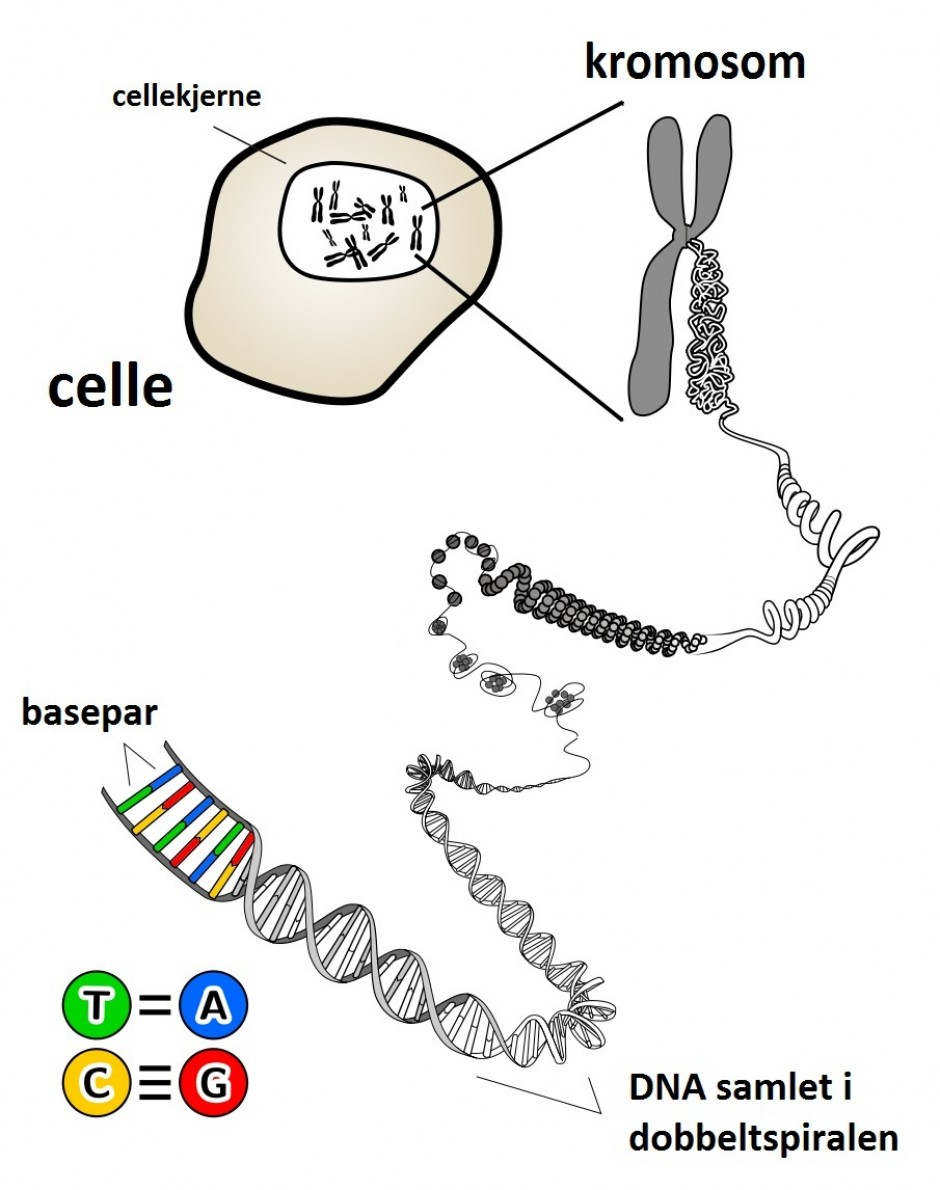
\includegraphics[scale = 0.20]{../figures/dna.jpg}
    \caption{Kromosom i cellekjernen. Kilde: forskning.no}
    \end{subfigure}
    \caption{Oppbygging av celler}
    \label{fig:celler}
\end{figure}

\subsection{Celleånding og Fotosyntese}
Levende celler er avhengig av energi for å kunne utføre cellens funksjoner, deriblant å kunne forflytte seg og reprodusere. En ku får i seg energi ved å beite på gress; mens andre organismer får i seg energi ved å spise andre dyr som spiser planter. Energien som lagres i mat kommer opprinnelig fra solen. Energi strømmer inn i et økosystem som sollys og går ut som varme; i motsetning, de kjemiske elementene som er essensielle for liv blir resirkulert. Fotosyntese generer oksygen og organiske molekyler som brukes av mitokondrier\footnote{En organell som finnes i de fleste celler, der de biokjemiske prosessene for celleånding og energi produksjon forekommer.} som brensel for celleånding. Avfallsproduktet fra celleåndingen er karbondioksid og vann, som igjen brukes i fotosyntese. Denne prosessen kan oppsummeres som følgende:
\begin{align*}
\text{Organisk materie} + \text{Oksygen} \longrightarrow \text{Karbondioksid} + \text{Vann} + \text{Energi}
\end{align*}

\subsection{Jordens utvikling}

\subsection{Miljø og naturen}

\end{document}